\section{Problem Setup and Background}
\mypara{Notations.}
Let $\inputs \subseteq \reals^{a_0 \times b_0 \times d_0}$ denote the space of inputs $\bfx$, where $d_0$ is the number of channels and $a_0$ and $b_0$ are the image size along each channel.
Let $\outputs := \{1, \cdots, L\}$ denote the space of output class labels $y$.
Let $\simplex_L$ denote the set of all probabilities over $\outputs$ (the simplex in $L$-dimensions).
We assume that natural inputs to the DNN classifier are sampled from an unknown probability distribution $\Pin$ over the space $\calX \times \outputs$.  
The  compact notation $[n]$ denotes $\{1, \cdots, n\}$ for a positive integer $n$.
Boldface symbols are used to denote both vectors and tensors.
$\langle\bfx, \bfx^\prime\rangle$ denotes the standard inner-product between a pair of vectors. 
% In the case of vectors, it is the standard $\bfx^T \,\bfx$. 
% In the case of image tensors $\bfx, \,\bfx^\prime \in \reals^{a \times b \times c}$, the inner-product is defined as the vector product along the third dimension. That is $\,\bfz = \langle\bfx, \bfx^\prime\rangle \in \reals^{a \times b}$ with $\,z_{ij} = \sum_{k=1}^c x_{ijk} \,x^\prime_{ijk}, ~i \in [a], j \in [b]$.
The indicator function $\indicator[c]$ takes value $1$ ($0$) when the condition $c$ is true (false).

\mypara{ID and OOD Datasets.}
% Throughout the paper, 
Consider a labeled ID training dataset $\Dintr = \{(\bfx_i, y_i), ~i = 1, \cdots, \Nintr\}$ sampled from the distribution $\Pin$.
We assume the availability of an unlabeled training dataset $\Douttr = \{\widetilde{\bfx}_i, ~i = 1, \cdots, \Nouttr\}$ from a different distribution, referred to as the {\em auxiliary OOD dataset}.
Similarly, we define the ID test dataset (from $\Pin$) as $\Dinte$, and the OOD test dataset as $\Doutte$.
Note that the auxiliary OOD dataset $\Dintr$ and the test OOD dataset $\Doutte$ are from different distributions.
All the OOD datasets are unlabeled since their label space is usually different from $\outputs$. 
% One can think of the OOD datasets for training, validation, and test to be biased samples from an unknown OOD marginal distribution $\Pout(\bfx)$.

\mypara{OOD Detector.}
%\label{sec:ood_detector}
The goal of an OOD detector is to determine if a test input to the classifier is ID (\ie from the distribution $\Pin$); otherwise the input is declared to be OOD~\citep{yang2021survey}.
Given a trained classifier $\bff : \calX \mapsto \Delta_L$, the decision function of an OOD detector can be generally defined as $\,\calD_\gamma(\bfx, \bff) \,=\, \indicator[S(\bfx, \bff) \geq \gamma]$, where $S(\bfx, \bff) \in \reals$ is the score function of the detector for an input $\bfx$ and $\gamma$ is the threshold.
%
\iffalse

Given a trained classifier $\bff$, the decision function of an OOD detector can be generally defined as~\citep{liu2020energy},
% \vspace{-3mm}
\begin{equation}
\label{eq:ood_detector}
\calD_\gamma(\bfx, \bff) ~=~ 
\begin{cases}
1, & \text{if } ~S(\bfx, \bff) \geq \gamma \\
0, & \text{otherwise }
\end{cases}
\end{equation}
where $S(\bfx, \bff) \in \reals$ is the score function of the detector for an input $\bfx \in \calX$, and $\gamma$ is the threshold.

\fi
%
We follow the convention that larger scores correspond to ID inputs, and the detector outputs of $1$ and $0$ correspond to ID and OOD respectively.
% For the brevity of notation, we use $\calD_\gamma(\bfx, \bff)$ and $\calD_\gamma$ interchangeably.
% Common choices for $S(\bfx, \bff)$ include the softmax confidence score (\ie the maximum predicted probability)~\citep{hendrycks2016msp}, the Energy score computed from logits at the penultimate layer~\citep{liu2020energy}, the negative maximum of the unnormalized logits~\citep{hendrycks2019scaling}, and other combined statistics from the intermediate feature representations~\citep{lee2018mahalanobis,raghuram2021JTLA}.
%It is worth noting that most of these methods for OOD detection can be modified to predict using the feature representation reconstructed from the concept space (\ie using $\recphi(\bfx)$). 
We assume the availability a pre-trained DNN classifier and a paired OOD detector that is 
trained to detect inputs for the classifier.

% \vspace{-0.1in}
\subsection{Projection Into Concept Space}
\label{sec:concept_projection}

% \begin{wrapfigure}{r}{0.5\linewidth}
\begin{figure}[ht]
\centering
% \rule{0.9\linewidth}{0.75\linewidth}
% \begin{figure}[t]
% \vspace{-0.2in}
% 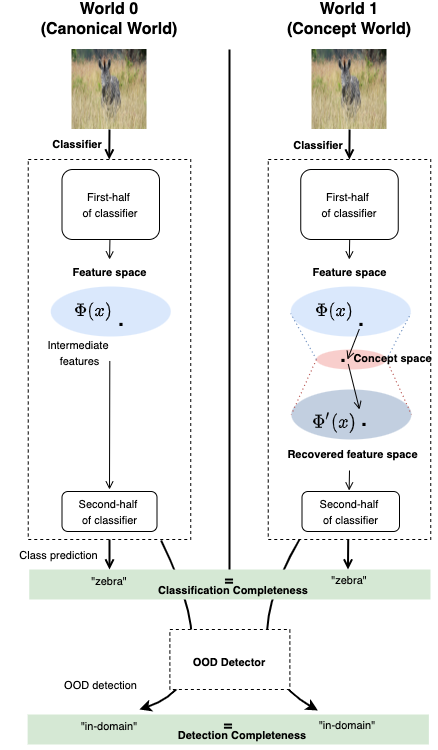
\includegraphics[width=0.45\textwidth]{figures/completeness.png}
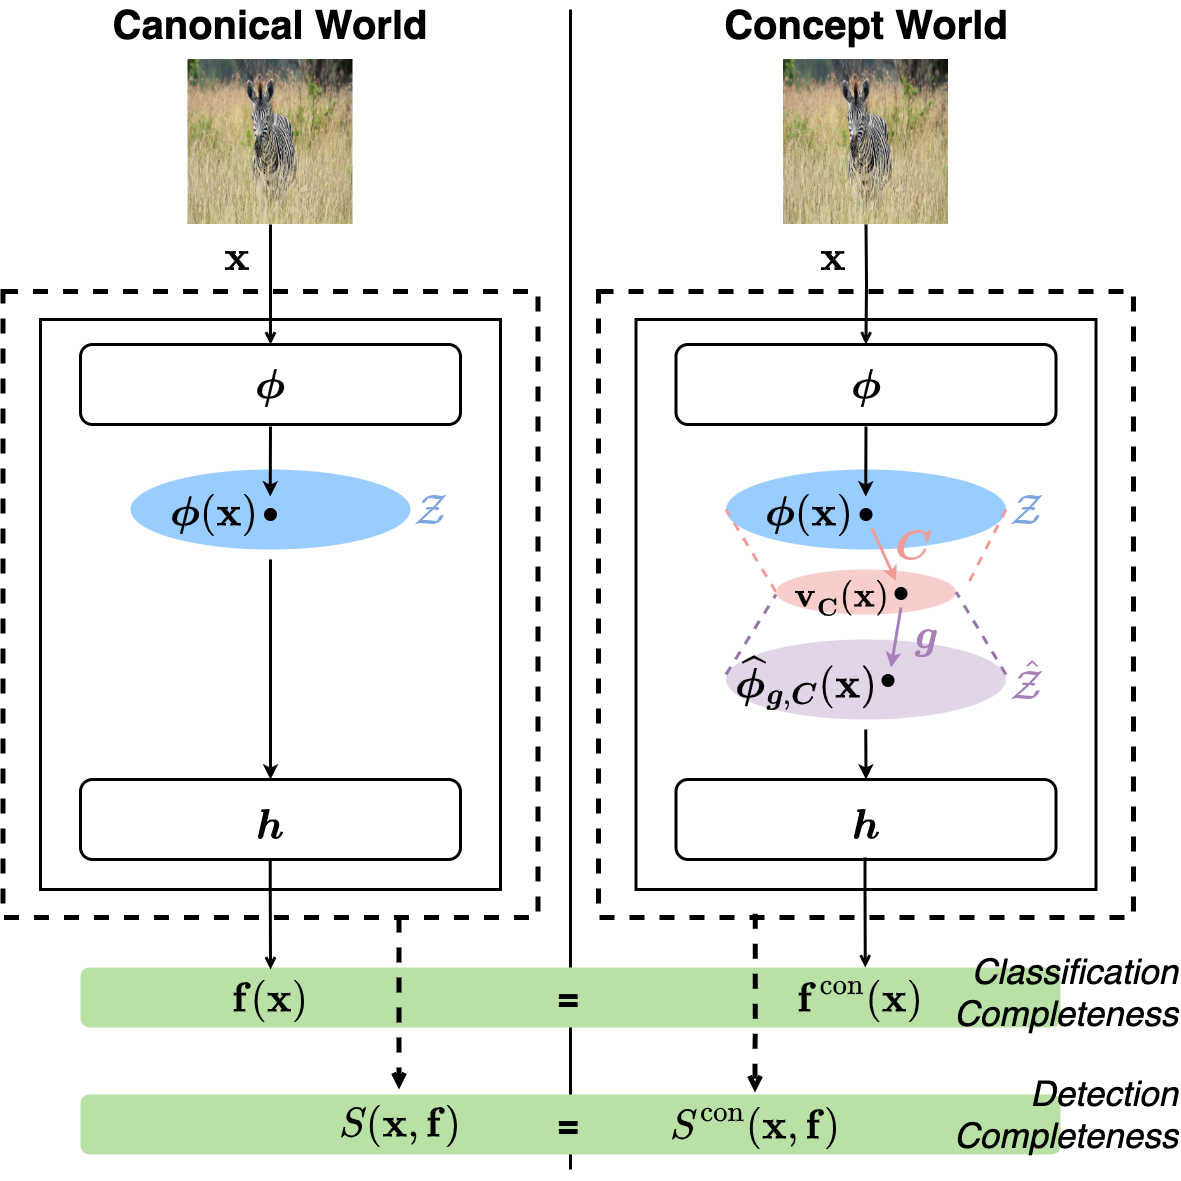
\includegraphics[scale=0.17]{figures/completeness_3.png} 
%\vspace{-2mm}
% \vspace{-0.2in}
\caption{
\textbf{Our two-world view of the classifier and OOD detector.} In the canonical world, both the classifier and OOD detector are unmodified. In the concept world, the layer representation $\bfphi(\bfx)$ is projected into the space spanned by the concept vectors and then reconstructed via the non-linear mapping $\bfg$. The classifier and OOD detector in the concept world are based on this reconstructed layer representation. Given the same input, the outputs from the DNN classifier and OOD detector in both the worlds should be very close to each other (characterized by \textit{Classification Completeness} and \textit{Detection Completeness}, respectively).
}
% \vspace{-3mm}
\label{fig:detection-completeness}
\vspace{-0.19in}
\end{figure}
% \end{wrapfigure}
%
\iffalse

\caption{\small \textbf{Our two-world view of the classifier and OOD detector.} Ideally, given the same input, the outputs both from the DNN classifier and OOD detector should be identical between the two worlds (characterized by \textit{Classification Completeness} and \textit{Detection Completeness}, respectively.)}

\begin{figure}[t]
\centering
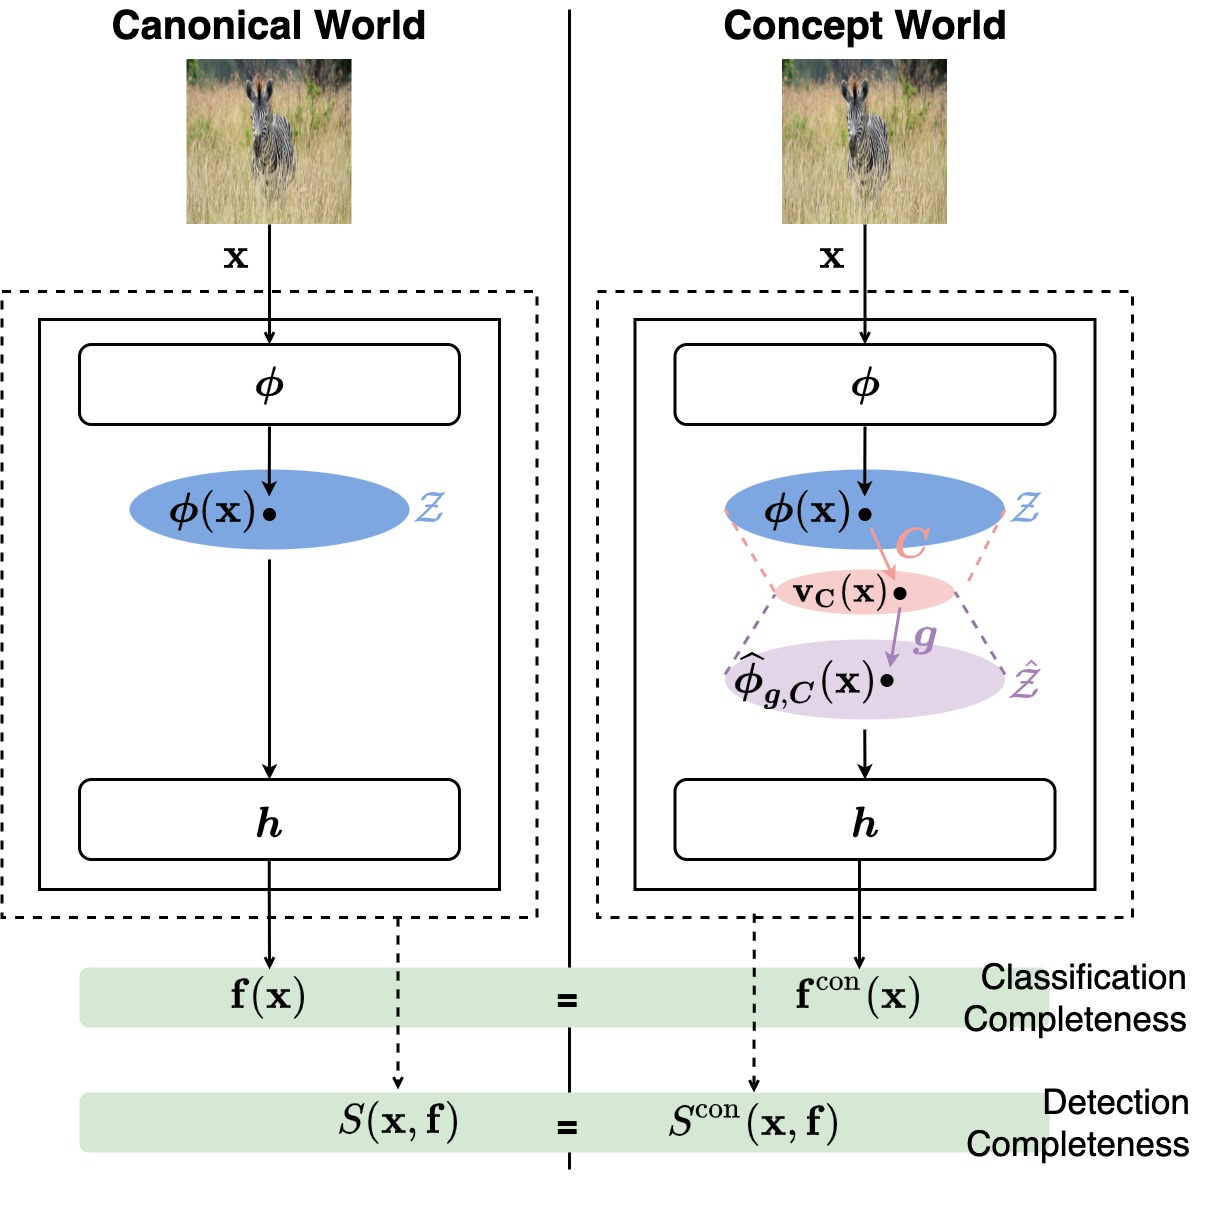
\includegraphics[scale=0.17]{figures/completeness_3.jpeg} 
\caption{\textbf{Our two-world view of the classifier and OOD detector.}}
\label{fig:detection-completeness}
\end{figure}

\fi

Consider a pre-trained DNN classifier $\bff : \mathcal{X} \mapsto \simplex_L$ that maps an input $\bfx$ to its corresponding predicted class probabilities. 
Without loss of generality, we can partition the DNN at a convolutional layer $\ell$ into two parts, \ie $\bff = \bfh \circ \bfphi$ where: 1) $\bfphi : \inputs \mapsto \calZ := \reals^{a_\ell b_\ell \times d_\ell}\,$ is the first half of $\bff$ that maps an input $\bfx$ to the intermediate feature representation~\footnote{We flatten the first two dimensions of the feature representation, thus changing an $a_\ell \times b_\ell \times d_\ell$ tensor to an $a_\ell b_\ell \times d_\ell$ matrix, where $a_\ell$ and $b_\ell$ are the filter size and $d_\ell$ is the number of channels.} $\bfphi(\bfx)$, and 2) $\bfh : \calZ \mapsto \simplex_L$ is the second half of $\bff$ that maps $\bfphi(\bfx)$ to the predicted class probabilities $\bfh(\bfphi(\bfx))$.
% For the feature representation at layer $\ell$, $d_\ell$ is the number of channels and $a_\ell$ and $b_\ell$ are the filter size (\eg $d_\ell = 2048$, $a_\ell = b_\ell = 5$ at the layer right before the global-pooling layer of the Inception-v3 network~\citep{szegedy2016inception-v3}).
We denote the predicted probability of a class $y$ by $\,f_y(\bfx) = h_y(\bfphi(\bfx))$, and the prediction of the classifier by $\,\widehat{y}(\bfx) = \argmax_{y} f_y(\bfx)$.

% \ap{I  brought in some stuff from Concept  Scores para in Section 3 to the following para to avoid duplication and ensure consistency. But, more I read it, I think the entire para on Concept Scores from there should be merged here. It is not clear by the way whether concept scores is from prior art or we are introducing it. No cites are given.}

Our work is based on the common implicit assumption of linear interpretability in the concept-based explanation literature, \ie high-level concepts lie in a linearly-projected subspace of the feature representation space $\calZ$ of the classifier~\citep{kim2018tcav}. 
% We explore the setting where high-level concepts lie in a subspace of the feature-representation space $\calZ$ of the classifier. 
% The feature representation is typically high-dimensional, \eg at the layer right before the global-pooling layer of the Inception-V3 network~\citep{szegedy2016inception-v3}, the dimension would be $25 \times 2048$ ($d_\ell = 2048, \,a_\ell = b_\ell = 5$).
Consider a projection matrix $\,\bfC = [\bfc_1, \cdots, \bfc_m] \in \reals^{d_\ell \times m}$ (with $m \ll d_\ell$) that maps from the space $\calZ$ into a reduced-dimension concept space. 
$\bfC$ consists of $m$ unit vectors, where $\bfc_i \in \reals^{d_\ell}$ is referred to as the \textit{concept vector} representing the $i$-th concept (\eg ``stripe'' or ``oval face''), and $m$ is the number of concepts.
% Based on the assumption that high-level concepts lie in a subspace of a feature-representation space of the classifier, consider a projection $\bfC \in \reals^{d_\ell \times m}$ (with $m \ll d_\ell$) that maps from the feature space into a reduced-dimension concept space (\eg a striped pattern). 
% \ryan{could be worth expanding on what the concepts could be since "stripe" can be ambiguous if the reviewers fail to connect it with figure 1}.
% We define the linear projection of a high-dimensional layer representation $\bfphi(\bfx) \in \reals^{a_\ell b_\ell \times d_\ell}$ into the concept space by $\,\VC(\bfx) := \bfphi(\bfx)\, \bfC \,\in \reals^{a_\ell b_\ell \times m}$. 
We define the \textit{concept score} for $\bfx$ as the linear projection of the high-dimensional layer representation $\bfphi(\bfx) \in \reals^{a_\ell b_\ell \times d_\ell}$ into the concept space~\citep{yeh2020completeness}, i.e. $\,\VC(\bfx) := \bfphi(\bfx)\, \bfC \,\in \reals^{a_\ell b_\ell \times m}$.
% This is referred to as the \textit{concept score} for $\bfx$ corresponding to the projection matrix $\bfC$~\citep{yeh2020completeness}.
% \ap{Is this our definition of concept score? Else we should cite prior art.}
% That is, $\bfv_{\bfC}(\bfx) := \bfC \bfphi(\bfx)$ is the \textit{concept score} for $\bfx$ defined by the projection matrix $\bfC$.
We also define a mapping from the projected concept space back to the feature space by a non-linear function $\,\bfg : \reals^{a_\ell b_\ell \times m} \mapsto \reals^{a_\ell b_\ell \times d_\ell}$.
% We define this reconstruction of the feature representation at layer $\ell$ from the concept space by $\,\recphi(\bfx) \,:=\, \bfg(\VC(\bfx))$.
The reconstructed feature representation at layer $\ell$ is then defined as $\,\recphi(\bfx) \,:=\, \bfg(\VC(\bfx))$.
% We note that $\bfg$ could be non-linear.
% To be precise, let $\,\recphi(\bfx) = \bfg(\VC(\bfx))$ define the reconstructed feature representation.
%Note that any DNN classifier can be modified to make predictions based on the reconstructed feature representation instead of the original feature representation.


% \vspace{-.1in}
\subsection{Canonical World and Concept World}
\label{sec:two_worlds}
% \mypara{Canonical World and Concept World.}
As shown in Fig.~\ref{fig:detection-completeness}, we consider a ``two-world'' view of the classifier and OOD detector consisting of the {\em canonical world} and the {\em concept world}, which are defined as follows:

\mypara{Canonical World.}
In this case, both the classifier and OOD detector use the original layer representation $\bfphi(\bfx)$ for their predictions. The prediction of the classifier is $\,\bff(\bfx) = \bfh(\bfphi(\bfx))$, and the decision function of the detector is $\,\calD_\gamma(\bfx, \bfh \circ \bfphi)$ with a score function $S(\bfx, \bfh \circ \bfphi)$.

% \mypara{\textbf{World 1 (\textit{concept world}).}}
\mypara{Concept World.}
% In this world, both the class prediction and OOD detection are based on the reconstructed feature representation $\recphi(\bfx)$ as shown in the right half of Fig.~\ref{fig:detection-completeness}.
We use the following observation in constructing the concept-world formulation: {\em both the classifier and the OOD detector can be modified to make predictions based on the reconstructed feature representation}, \ie using $\recphi(\bfx)$ instead of $\bfphi(\bfx)$. 
% This idea is illustrated in the right half of Fig.~\ref{fig:detection-completeness}. 
Accordingly, we define the corresponding classifier, detector, and score function in the concept world as follows:
\begin{align}
\label{equ:concept_world}
\centering
\fcon(\bfx) ~&:=~ \bfh(\recphi(\bfx)) ~=~ \bfh(\bfg(\VC(\bfx))) \nonumber \\
\Dcon(\bfx, \bff) \,&:=\, \calD_\gamma(\bfx, \bfh \circ \recphi) \,=\, \calD_\gamma(\bfx, \bfh \circ \bfg \circ \VC) \nonumber \\
\centering
\Scon(\bfx, \bff) \,&:=\, S(\bfx, \bfh \circ \recphi) \,=\, S(\bfx, \bfh \circ \bfg \circ \VC).
\end{align}
%
%1) {\em canonical world}, where both the classifier and detector use the original layer representation $\bfphi(\bfx)$ for their predictions; 
%2) {\em concept world}, where both the classifier and detector use the concept score-based reconstruction of the layer representation $\recphi(\bfx)$ for their predictions. 
%
We further elaborate on this two-world view and introduce the following two desirable properties.
% , viz. detection completeness and concept separability.

% Such observation gives rise to two worlds where a DNN classifier and an OOD detector can be in (outlined in Figure \ref{fig:detection-completeness}):
% % This is the starting point of our work.
% \jihye{formatting the following two paragraphs: indent/list?}

% \mypara{\textbf{World 0 (\textit{canonical world}).}} 

%
\mypara{Detection Completeness.} Given a fixed algorithmic approach for learning the classifier and OOD detector, and with fixed internal parameters of $\bff$, we would ideally like the classifier prediction and the detection score to be indistinguishable between the two worlds. 
In other words, for the concepts to \textit{sufficiently} explain the OOD detector, we require $\Dcon(\bfx, \bff)$ to closely mimic $\calD_\gamma(\bfx, \bff)$. 
Likewise, we require $\fcon(\bfx)$ to closely mimic $\bff(\bfx)$ since the detection mechanism of $\calD_\gamma$ is closely paired to the classifier.
We refer to this property as the {\em completeness of a set of concepts with respect to the OOD detector and its paired classifier.}  
% As discussed in \S~\ref{sec:completeness_score}, this extends the notion of classification completeness introduced by~\citet{yeh2020completeness} for a classifier to a pair consisting of both the OOD detector along with its paired classifier.
As discussed in \S~\ref{sec:completeness_score}, this extends the notion of classification completeness introduced by~\citet{yeh2020completeness} to an OOD detector and its paired classifier.
% This translates to finding an optimal set of concept vectors $\bfC$ and a reconstruction network $\bfg$ to achieve the above goals.


\iffalse

We assume that with a fixed algorithmic approach for $\calD$ and a fixed internals of $\bff$, the classifier output and detection score should be indistinguishable between the two worlds.
In other words, for concepts to \textit{sufficiently} explain an OOD detector, $\Dcon(\bfx, \bff)$ should mimic $\calD_\gamma(\bfx, \bff)$ sufficiently well. 
Likewise, we require $\fcon(\bfx)$ to imitate $\bff(\bfx)$ sufficiently well, as the algorithm of $\calD$ is paired with $\bff$.
If the performance gap between the two worlds is large, one should not trust that the explanations resulted from $\bfC$ are accurate description of the target detector $\calD$.

To improve the interpretability of the resulting explanations, we impose another important property on the learned concepts: data detected as ID by $\calD_\gamma$ (henceforth referred to as \textit{ID-detected} data) and data detected as OOD by $\calD_\gamma$ (henceforth referred to as \textit{OOD-detected} data) should be well separated in the concept space.
Refer to Figure \ref{fig:detection-separability} for illustration purposes.
While the ID input and OOD input show clear distinctive patterns for concept "Stripe" and "Oval Face", concept "Sky" and "Greenery" would decrease the overall distinction between the two inputs in terms of concepts. 
The four concepts might be sufficient to close the gap between canonical world and concept world, but considering that our work aims to guide humans to understand what concepts distinguish ID data and OOD data, we would prefer a set of concepts that have well-separated pattern for different detection outputs.

\fi

\mypara{Concept Separability.} To improve the interpretability of the resulting explanations for the OOD detector, we require another desirable property from the learned concepts: data detected as ID by $\calD_\gamma$ (henceforth referred to as \textit{detected-ID} data) and data detected as OOD by $\calD_\gamma$ (henceforth referred to as \textit{detected-OOD} data) should be well-separated in the concept-score space.
Since our goal is to help an analyst understand which concepts distinguish the detected-ID data from detected-OOD data, we would like to learn a set of concepts that have a well-separated concept score pattern for inputs from these two groups (\eg the concepts $C_{90}$ and $C_1$ in Fig.~\ref{fig:expl-ours-dolphin} have distinct concept scores).
% Going back to Fig.~\ref{fig:detection-separability} for illustration, 
% While the concepts ``stripe'' and ``oval face'' show clear distinctive patterns between the inputs, concepts ``sky'' and ``greenery'' have a similar concept-score pattern. 
% , even when their class predictions are identical.
% for different detection outputs.

%Include the following para if space permits.
%In summary, we identify two desirable properties for the learned concepts in order to explain the OOD detector sufficiently well: (1) Detection completeness: the concept scores are essentially sufficient statistics for recovering the performance of the OOD detector and its paired classifier in the concept world; and (2)  Concept separability: for improved interpretability of the detector, the detected-ID data and detected-OOD data should have clearly-distinctive patterns in the concept world. 
% We next propose a method for learning such concepts.

\iffalse

In summary, we identify two desirable properties for the learned concepts in order to explain the OOD detector sufficiently well: (1) Detection completeness:  The concept scores are essentially sufficient statistics for recovering the performance of the OOD detector (\eg area under the ROC curve) and its paired classifier (\eg accuracy) in the concept world; and (2)  Concept separability: For improved interpretability of the detector, the detected-ID data and detected-OOD data should have clearly-distinctive patterns in the concept world. We next propose a method for learning such concepts.
% \jihye{using detector as oracle.}

\fi



